\chapter[Improving Deep Neural Networks]{Improving Deep Neural Networks\setcounter{footnote}{0}\footnote{Hyperparameter Tuning, Regularization and Optimization}}

%%%
\section{Setting up and Regularizing neural network}

在本章中会引入一些新的符号,如表~\ref{tab:notations-chap2} 所示。

\begin{table}[htb!]
    \centering
    \begin{threeparttable}
    %%
    \caption{Appended Notations in Chapter 2}
    %
    \begin{tabular}{clcc}
        \toprule
                                    & \textbf{Notation}                                                                     & \textbf{Description} & \textbf{Meaning}                                                   \\ 
        \midrule
        \multirow{1}{*}{Sizes}      & $\verb|batch_size| \in \mathbb{Z}^+$								                    & value                & 每个 \verb|mini_batch| 使用的样本数          \\
        \midrule
        \multirow{5}{*}{Objects}    & $X^{\{t\}} \in \mathbb{R}^{n_x \times \mathtt{batch\_size}}$                          & matrix               & 第$t$个 \verb|mini_batch| 的输入矩阵                                                               \\
                                    & $Y^{\{t\}} \in {\mathbb{R}^{n_y \times \mathtt{batch\_size}}}$                        & matrix               & 第$t$个 \verb|mini_batch| 的样本标签矩阵                                                           \\									
                                    & $\hat{Y}^{\{t\}} / A^{[L]\{t\}} \in {\mathbb{R}^{n_y \times \mathtt{batch\_size}}}$   & matrix               & 第$t$个 \verb|mini_batch| 的标签预测值矩阵   						\\
                                    & $v_{\d \mathrm{var}}$                                                                 & matrix               & 梯度 $\d \mathrm{var}$ 第一矩估计的移动平均值                                 \\
                                    & $s_{\d \mathrm{var}}$                                                                 & matrix               & 梯度 $\d \mathrm{var}$ 第二矩估计的移动平均值                                 \\
        \midrule
        \multirow{6}{*}{Other}      & $\lambda \in \mathbb{R}^+_0$                                                          & value                & 正则化参数                                                             \\  
                                    & \verb|keep_prob| $\in [0,1]$                                                          & value                & Dropout算法的保留概率                                                      \\ 
                                    & $J^{\{t\}}$                                                                           & function             & 第$t$个 \verb|mini_batch| 的代价函数                                                                        \\  
                                    & $\beta_1 \in [0,1]$                                                                   & value                & 第一矩估计的衰减率 \\ 
                                    & $\beta_2 \in [0,1]$                                                                   & value                & 第二矩估计的衰减率                                                    \\ 
                                    & $\varepsilon \in \mathbb{R}^+$                                                        & value                & 第二矩估计中的数值稳定性参数                                                    \\
        \bottomrule
    \end{tabular}
    %
    \label{tab:notations-chap2} %
    \begin{tablenotes}
        \item[*] 通常情况下${\{t\}}$表示第$t$个batch。
    \end{tablenotes}
    %%
    \end{threeparttable}
\end{table}

%%%%
\subsection{Train/Dev/Test sets}
对于数据集,我们通常将其分为三个部分:
\begin{itemize}
    \item \textbf{Training set}: 训练集,用于训练模型。一般占60\%。
    \item \textbf{Dev (development) set}: 开发集,用于调整模型的超参数。一般占20\%。
    \item \textbf{Test set}: 测试集,用于测试模型的性能。一般占20\%。
\end{itemize}
有时候,我们会将数据集仅分为训练集和开发集,而没有测试集。这时候,我们通常将二者的比例调整为70\%和30\%。

%%%%
\subsection{Bias and Variance}
\textbf{偏差(Bias)}描述了模型的预测值与真实值之间的差距。Bias越大,说明模型越不准确。
而\textbf{方差(Variance)}描述了模型的预测值与真实值之间的差距的方差。Variance越大,说明模型越不稳定。

\begin{figure}[h!bt]
    \centering
    \subfigure[High Bias]{
        \begin{minipage}[t]{0.3\textwidth}
            \centering
            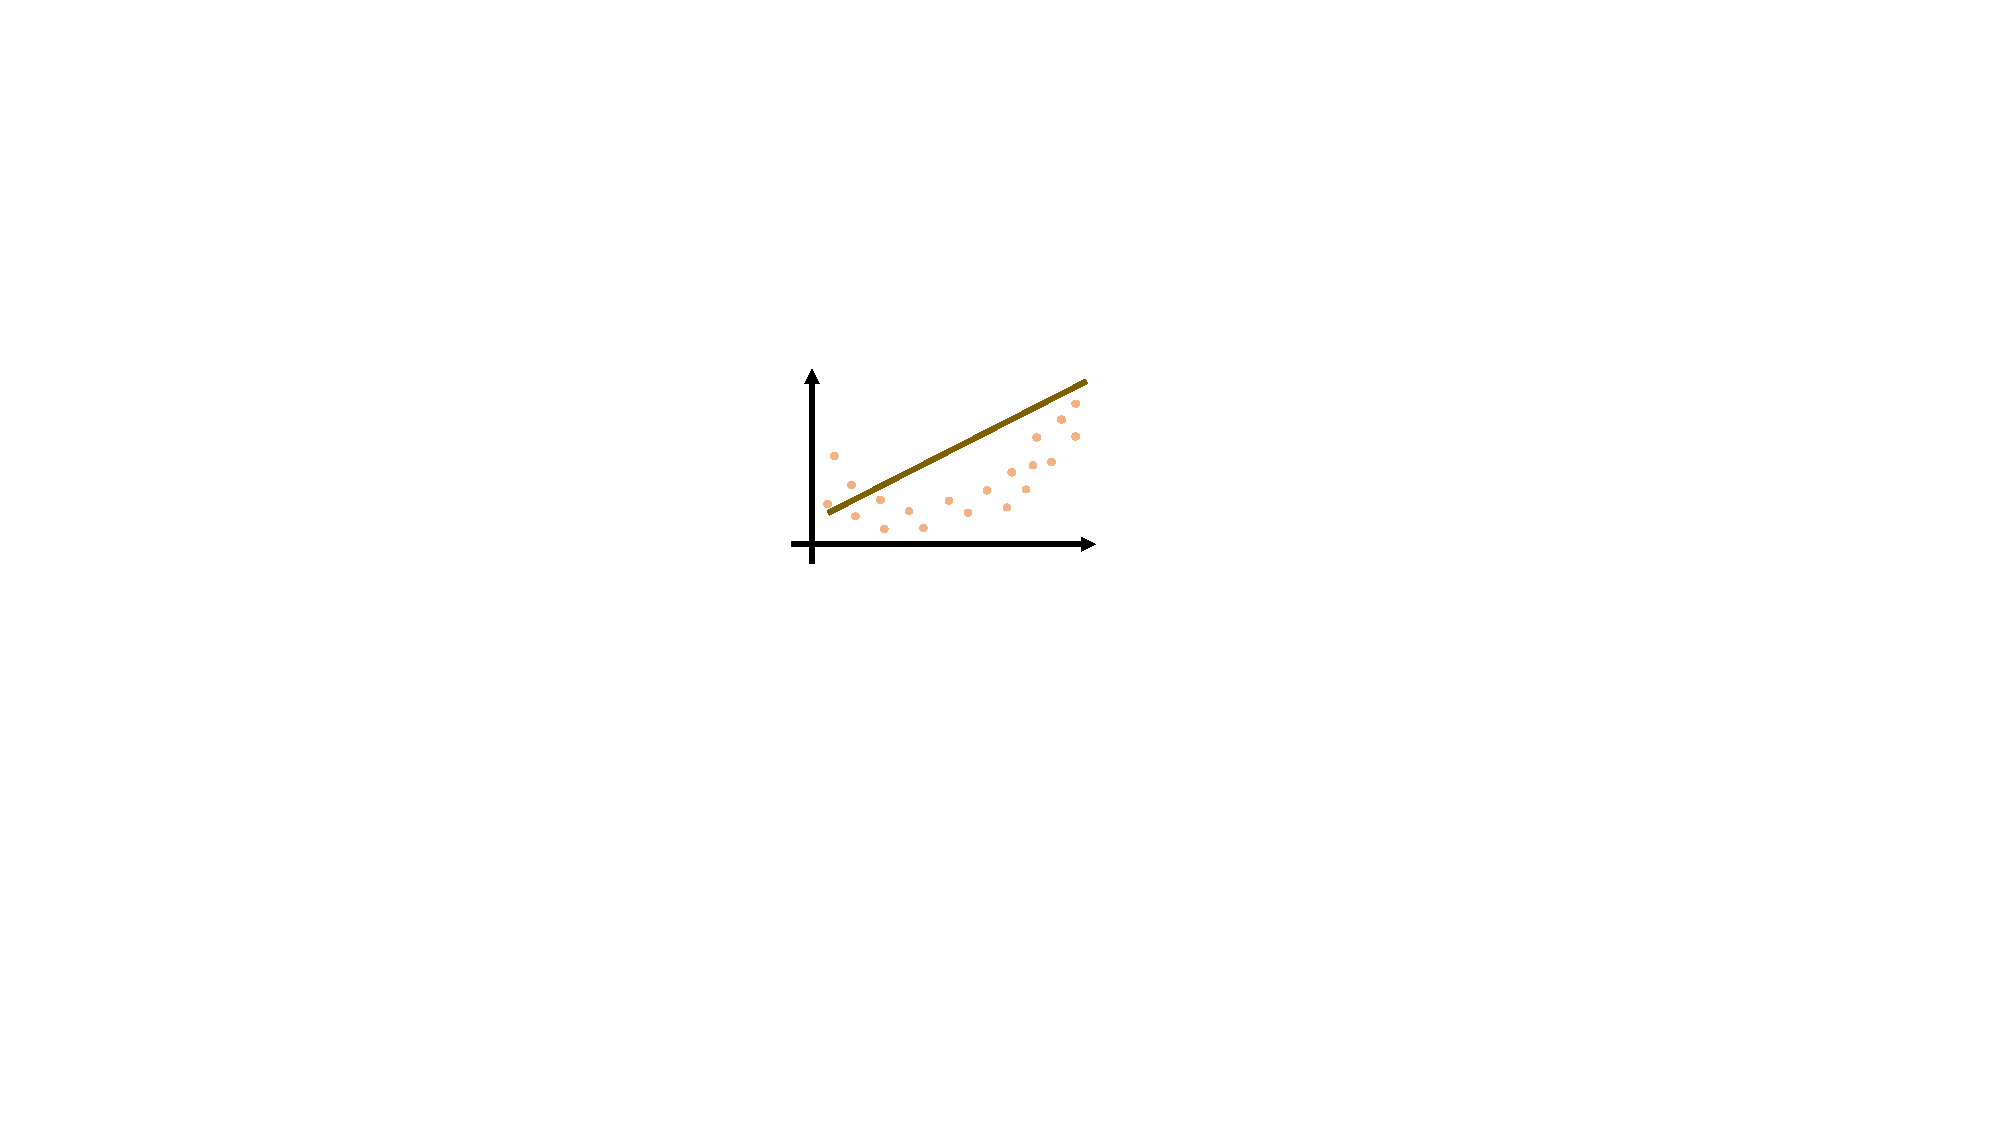
\includegraphics[scale=0.75]{high_bias.pdf}
        \end{minipage}
    }%
    \subfigure[Just Right]{
        \begin{minipage}[t]{0.3\textwidth}
            \centering
            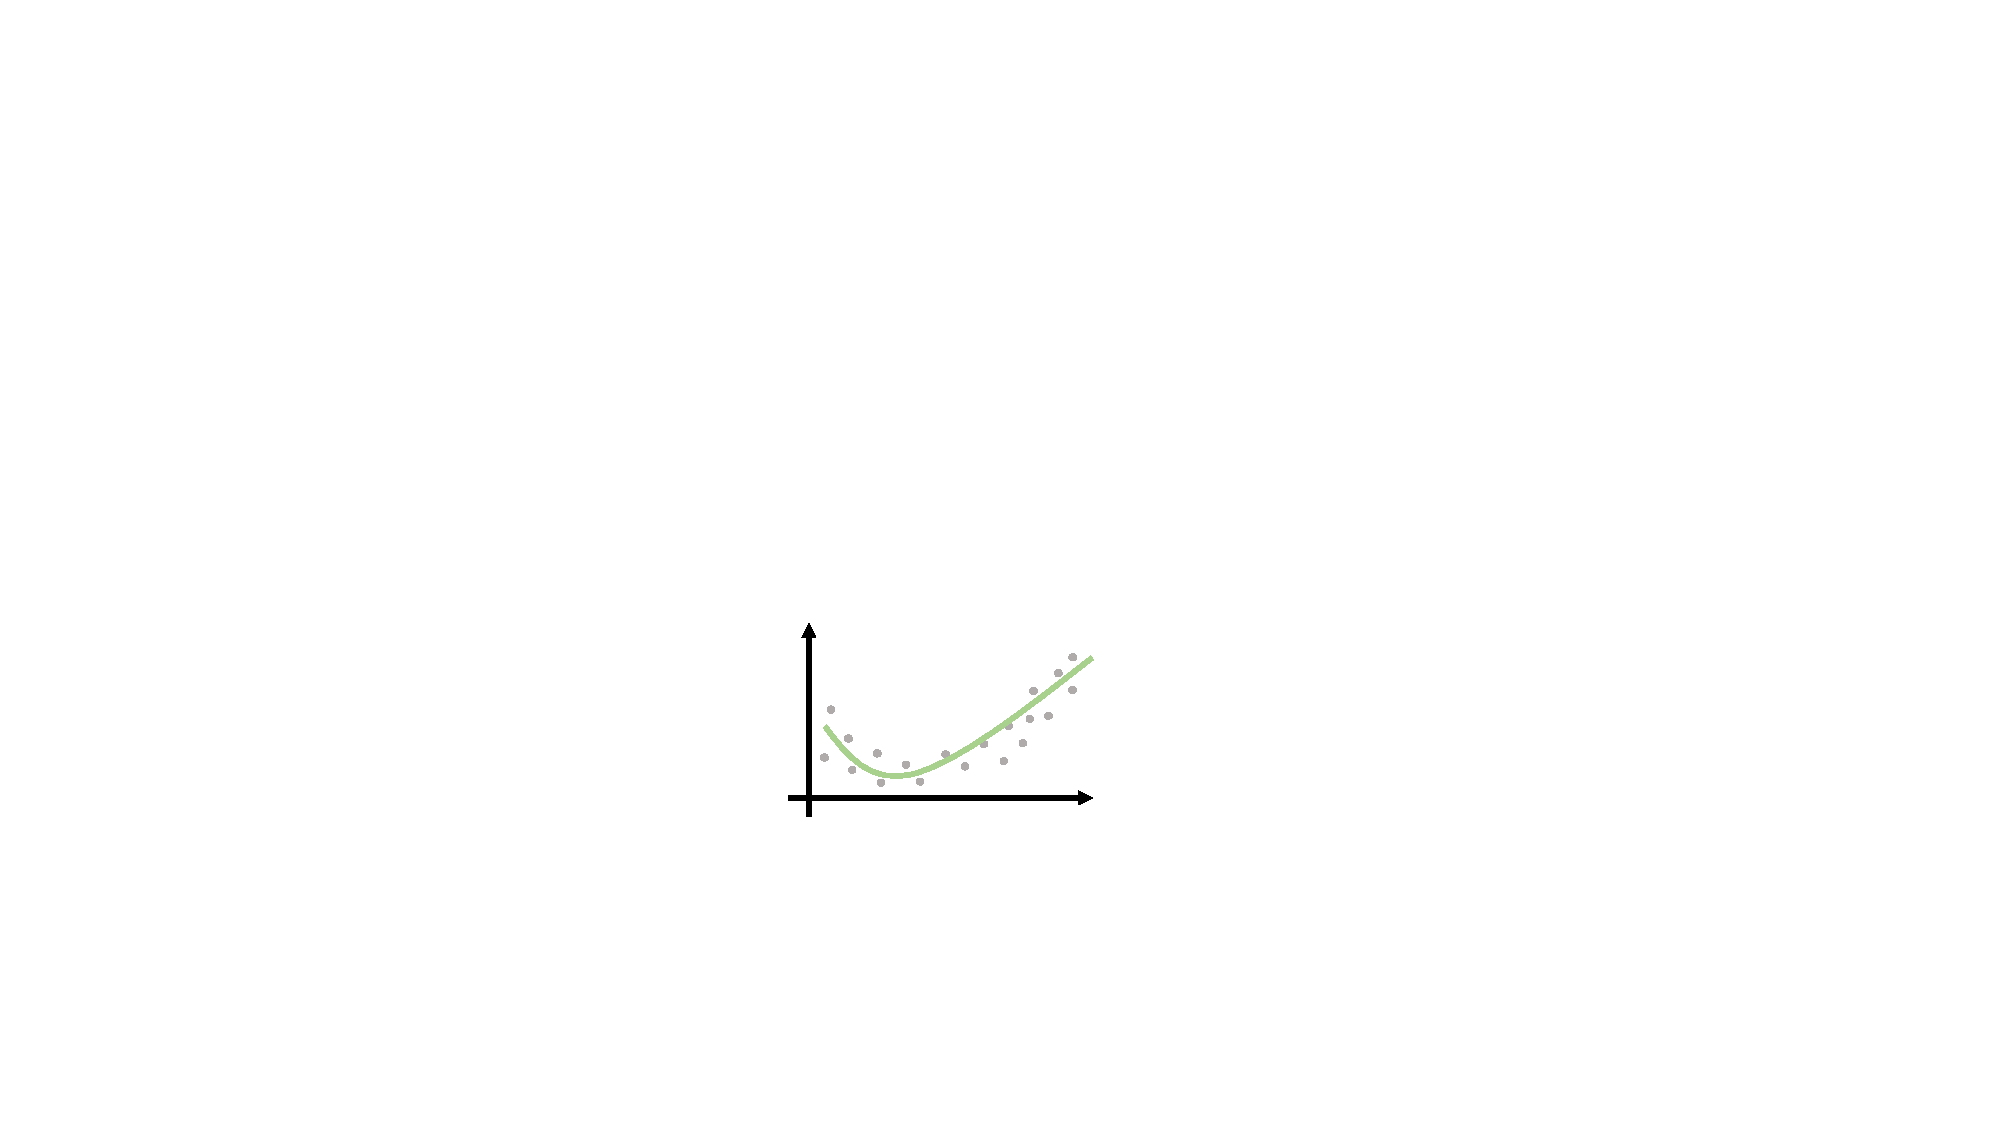
\includegraphics[scale=0.75]{just_right.pdf}
        \end{minipage}
    }%
    \subfigure[High Variance]{
        \begin{minipage}[t]{0.3\textwidth}
            \centering
            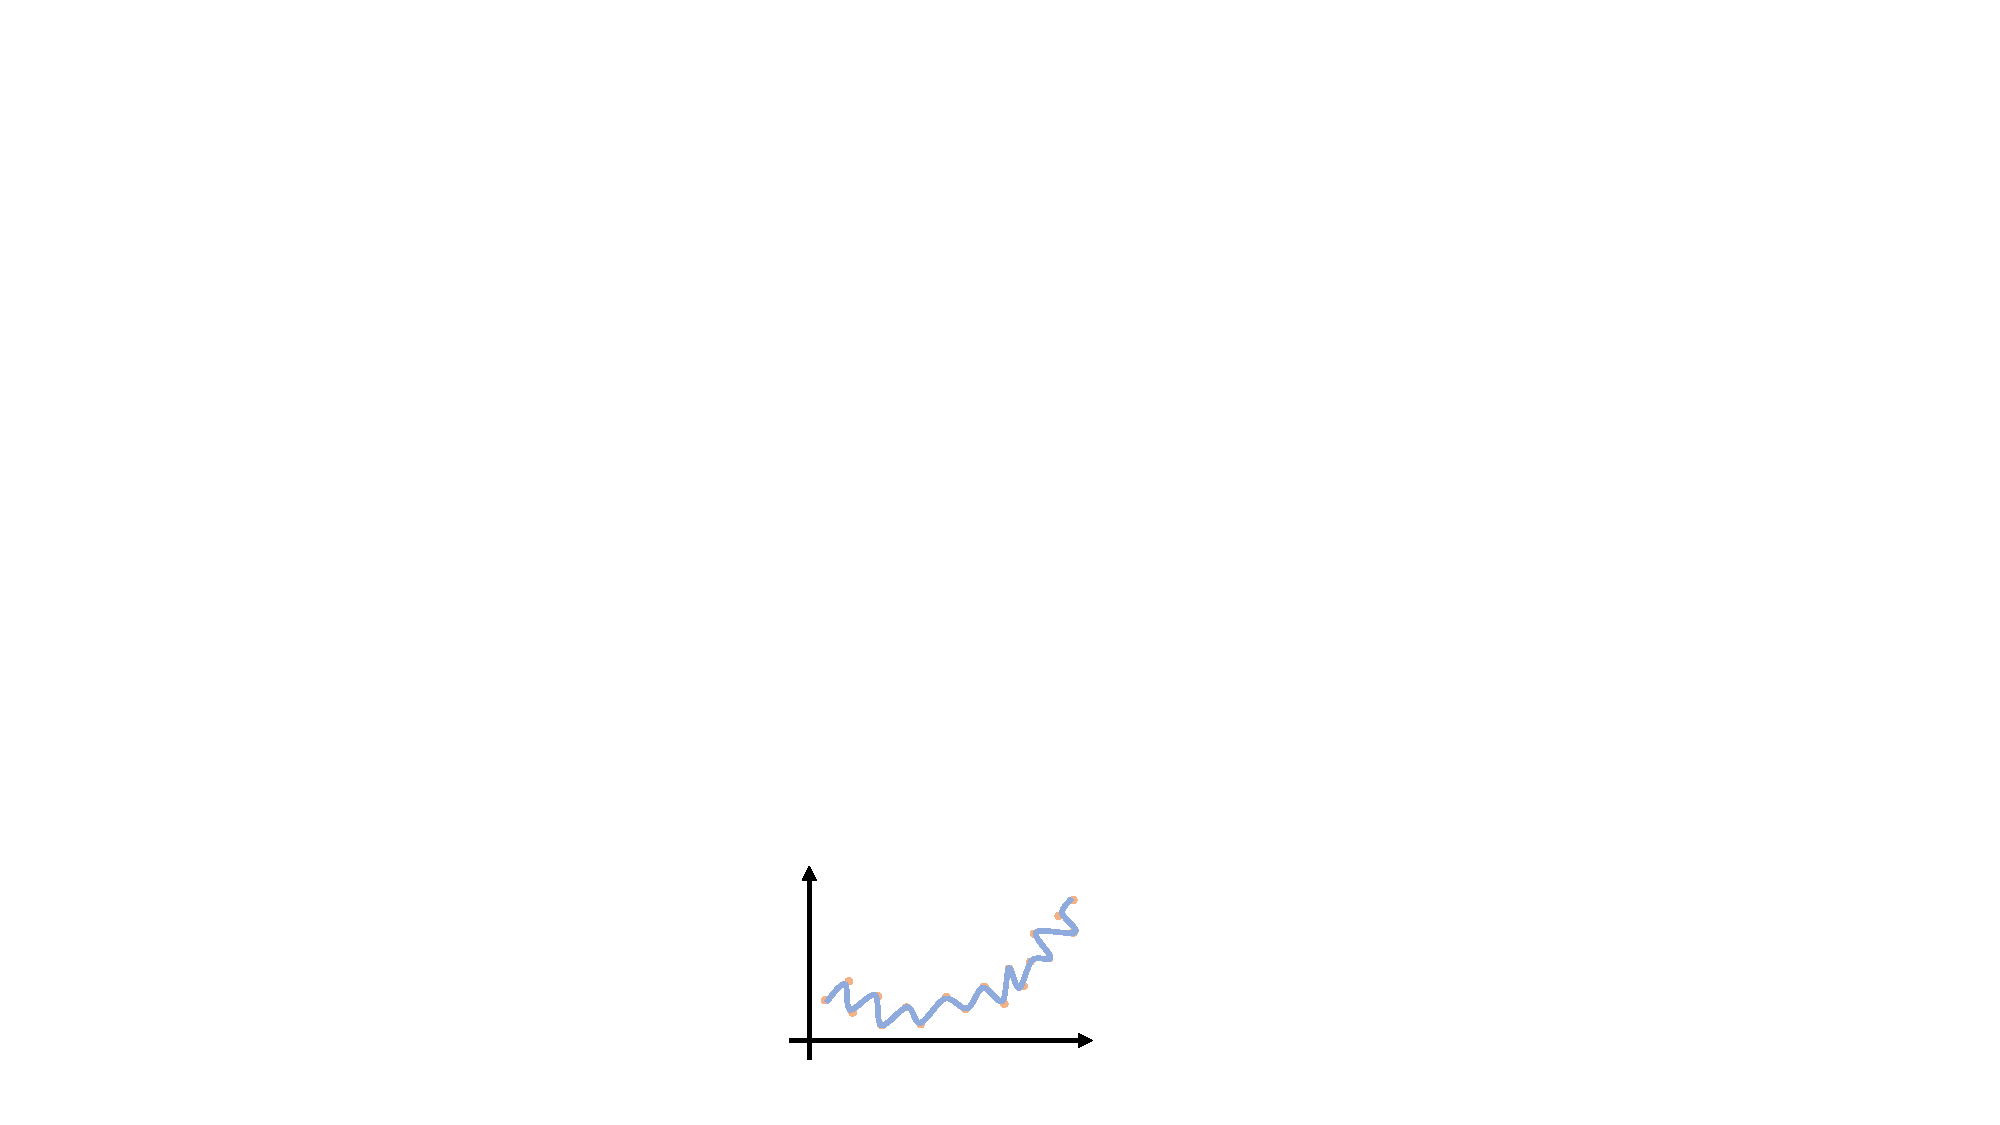
\includegraphics[scale=0.75]{high_variance.pdf}
        \end{minipage}
    }%
    \centering
    \caption{Bias and Variance}
    \label{fig:bias-variance}
\end{figure}

\textbf{高偏差(High bias)}通常表示模型欠拟合,即模型的复杂度不够,无法拟合数据。这可以体现在模型在训练集上的误差和在开发集上的误差都很大,且二者之间的差距不大。
而\textbf{高方差(High variance)}通常表示模型过拟合,即模型的复杂度过高,导致模型过于敏感,无法泛化。这可以体现在模型在训练集上的误差很小,但在开发集上的误差很大。
若高偏差和高方差同时存在,则会体现在模型在训练集上的误差和在开发集上的误差都很大,且开发集上的误差明显大于训练集上的误差。

当我们发现模型的偏差很大时,可以尝试使用更大的网络、训练更长的时间、使用更好的优化算法等来提高模型的复杂度,从而减小偏差。
而当我们发现模型的方差很大时,可以尝试使用更多的数据、使用正则化、使用dropout等来减小模型的复杂度,从而减小方差。

%%%%
\subsection{Regularization}
\index{Regularization}

正则化(Regularization)是一种减小模型复杂度的方法,可以防止模型过拟合。
正则化的方法有很多,这里介绍两种常用的正则化方法:$L_2$正则化和Dropout。

\begin{hint}
    正则化的目的是改变(通常是缩小)在更新权重和偏置时的梯度值,其本身并不干预模型的前向传播和反向传播过程。
\end{hint}

\subsubsection{$\mathsf{L_2}$ regularization}

$L_2$正则化($L_2$ regularization)也称为权重衰减(Weight Decay),是一种常用的正则化方法。
$L_2$正则化通过在代价函数中添加一个权重
\footnote{一般不对偏置做$L_2$正则化,避免影响神经元的激活阈值。}
的$L_2$范数
\footnote{$L_2$范数是针对向量的,而Frobenius范数是针对矩阵的,在这里并没有做严谨的区分。}
惩罚项来实现,这个惩罚项模型权重的平方成正比。这样做的目的是鼓励模型使用较小的权重,从而减少模型的复杂度。

$L_2$范数的定义是,对于一个长度为$n$的向量$w$,其$L_2$范数为:
\begin{equation}
    ||w||_2 = \sqrt{\sum_{j=1}^nw_j^2}
\end{equation}

使用$L_2$正则化后,代价函数中添加了各层权重信息的Frobenius范数,其计算公式为:
\begin{equation}
    J = \frac{1}{m}\sum_{i=1}^mL(\hat{y}^{(i)}, y^{(i)}) + \frac{\lambda}{2m}\sum_{l=1}^L||W^{[l]}||_{\mathrm{F}}^2
\end{equation}
其中$\lambda$为正则化参数,用于控制正则化的强度。$||W^{[l]}||_2^2$表示第$l$层权重Frobenius范数的平方,即
\begin{equation}
    ||W^{[l]}||_{\mathrm{F}}^2 = \sum_{i=1}^{n^{[l]}}\sum_{j=1}^{n^{[l-1]}}(W_{ij}^{[l]})^2
\end{equation}
添加这个惩罚项后,代价函数对权重的梯度为:
\begin{equation}
    \frac{\d J}{\d W^{[l]}} = \frac{\d J}{\d Z^{[l]}} A^{[l-1] \mathrm{T}} + \frac{\lambda}{m}W^{[l]}
\end{equation}
其他的梯度表达式保持不变(证明略)。

\subsubsection{Dropout}
\index{Dropout}

Dropout是一种常用的正则化方法,可以防止模型过拟合。Dropout的基本思想是,在每次迭代中,随机地关闭一些神经元,从而减小模型的复杂度,相当于只训练了完整模型的一个子集。
Dropout 是以层为单位来使用的,即在设定的某些 Dropout 层中,每次迭代时,以一定的概率关闭其中的神经元(每次迭代可以关闭不同的神经元)。

需要注意,“关闭”神经元并不是将神经元中的权重和偏置清零,而只是将其输出置零。

\begin{figure}[h!bt]
    \centering
    \subfigure[随机选取神经元]{
        \begin{minipage}[t]{0.48\textwidth}
            \centering
            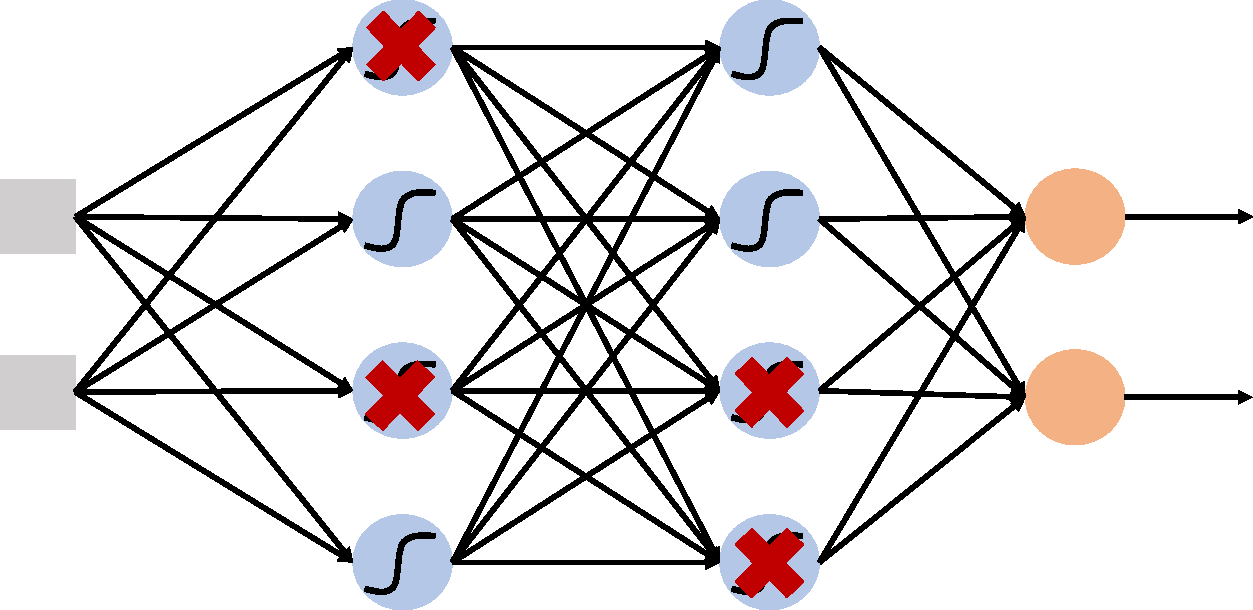
\includegraphics[width=0.8\textwidth]{dropout_1.pdf}
        \end{minipage}
    }%
    \subfigure[输出置零]{
        \begin{minipage}[t]{0.48\textwidth}
            \centering
            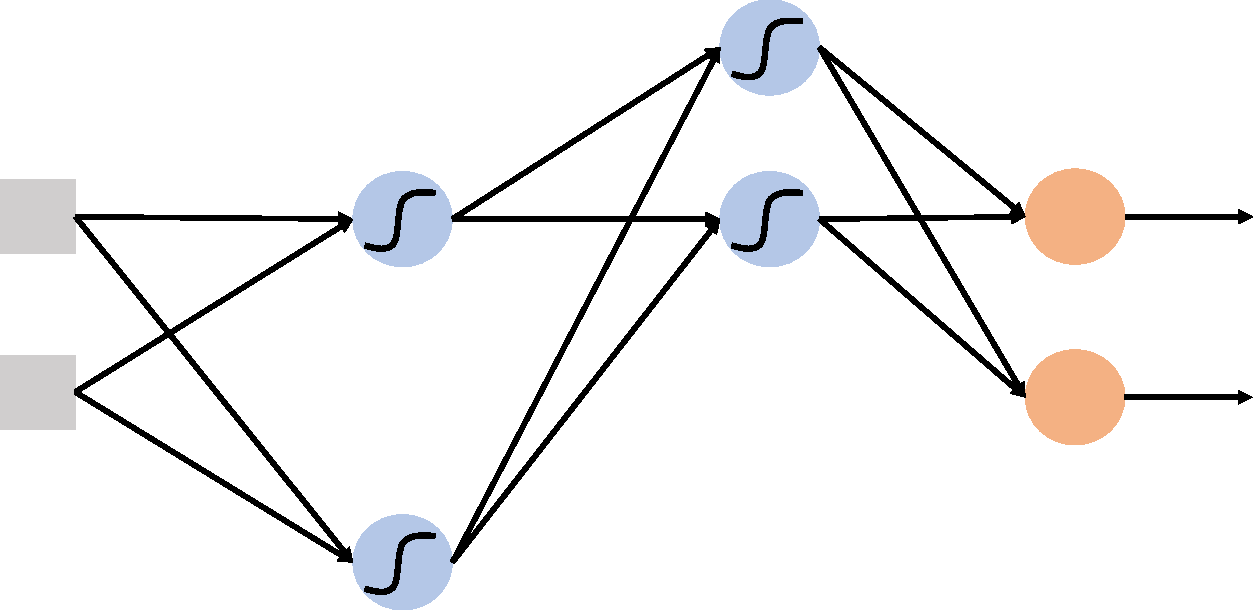
\includegraphics[width=0.8\textwidth]{dropout_2.pdf}
        \end{minipage}
    }%
    \centering
    \caption{Dropout}
    \label{fig:dropout}
\end{figure}

一种常见的Dropout实现为Inverted dropout。假设第$l$层被设置为Dropout层,设置一个保留概率 \verb|keep_prob| ,
则在每次迭代的前向传播中,先用原有的方式计算出第$l$层的激活值$A^{[l]}$,然后构造一个布尔矩阵(mask)$D^{[l]}$,其中的元素以概率 \verb|keep_prob| 取值为1,以概率 \verb|1-keep_prob| 取值为0。
\footnote{严格来说,“关闭”某些神经元应当将$A^{[l]} \in \mathbb{R}^{n^{[l]} \times {m}}$的某些行随机置零,而不是对所有元素随机置零。对所有元素随机置零相当于在同一轮迭代中每个样本都关闭了不同的神经元,但这样做也是可行的。}
\begin{equation}
    \mathtt{D^{\textcolor{Magenta}{[}l\textcolor{Magenta}{]}}} = \mathtt{np.random.rand\textcolor{yellow}{(} A^{\textcolor{Magenta}{[}l\textcolor{Magenta}{]}}.shape\textcolor{Magenta}{[}\textcolor{green}{0}\textcolor{Magenta}{]}, A^{\textcolor{Magenta}{[}l\textcolor{Magenta}{]}}.shape\textcolor{Magenta}{[}\textcolor{green}{1}\textcolor{Magenta}{]} \textcolor{yellow}{)} < keep\_prob}
\end{equation}
将这个布尔矩阵与$A^{[l]}$相乘,即可将第$l$层的部分输出置零
\begin{equation}
    \mathtt{A^{\textcolor{Magenta}{[}l\textcolor{Magenta}{]}}} = \mathtt{np.multiply\textcolor{yellow}{(} A^{\textcolor{Magenta}{[}l\textcolor{Magenta}{]}}, D^{\textcolor{Magenta}{[}l\textcolor{Magenta}{]}} \textcolor{yellow}{)}}
\end{equation}
为了补偿训练过程中由于 Dropout 导致的输出值的减少,需要进行一次缩放,即
\begin{equation}
    \mathtt{A^{\textcolor{Magenta}{[}l\textcolor{Magenta}{]}}} /= \mathtt{keep\_prob}
\end{equation}
将这个值作为第$l$层的输出$A^{[l]}$。这个操作应在计算第$l+1$层之前完成。

在反向传播中,使用这些经过 Dropout 的各层输出来计算梯度来更新权重和偏置。同时,$\d A^{[l]}$也需要进行类似的操作使其与$A^{[l]}$对应,即
\begin{align}
    \mathtt{dA^{\textcolor{Magenta}{[}l\textcolor{Magenta}{]}}} &= \mathtt{np.multiply\textcolor{yellow}{(} dA^{\textcolor{Magenta}{[}l\textcolor{Magenta}{]}}, D^{\textcolor{Magenta}{[}l\textcolor{Magenta}{]}} \textcolor{yellow}{)}} \\
    \mathtt{dA^{\textcolor{Magenta}{[}l\textcolor{Magenta}{]}}} &/= \mathtt{keep\_prob}
\end{align}
这个操作应在计算第$l-1$层之前完成。

从结果上看,Dropout 操作相当于这一轮迭代中的训练的神经元数“减少”了,这可以降低模型对单个神经元的依赖,从而提高模型的泛化能力。

在评估模型或者使用模型进行预测时(此时只有前向传播),需要关闭Dropout。这是为了确保模型的输出与训练阶段保持一致,从而准确评估模型在未见数据上的性能。

\subsubsection{Other regularization methods}

除了$L_2$正则化和Dropout,还有一些其他的正则化方法,如数据增强(Data Augmentation)、早停(Early Stopping)等。

数据增强是一种简单有效的正则化方法,其基本思想是通过对训练集中的数据进行一些随机变换,从而生成更多的训练数据。
例如,对于图像分类问题,可以对图像进行一些随机的旋转、平移、缩放等操作,将其作为新增的训练数据。

早停的基本思想是在训练过程中,当模型在开发集上的误差连续一段时间不再下降时,就停止训练。
这样可以防止模型过拟合,但需要注意的是,早停的效果很大程度上依赖于开发集的选择。

\subsection{Normalizing Inputs}
\index{Normalization}

在训练神经网络时,我们通常会对输入数据进行归一化处理。
归一化可以确保数值在可接受的范围内,将所有特征重现在相同的尺度上,提高算法的数值稳定性。

数据归一化通常包括两个步骤:减去平均值(使得归一化后的数据具有零均值)和除以标准差(使得归一化后的数据具有单位方差)。
这种方法也被称为 Z-score 标准化或标准化。在标准化后,数据的均值为0,标准差为1。

\begin{figure}[h!bt]
    \centering
    \subfigure[Before Normalization]{
        \begin{minipage}[t]{0.48\textwidth}
            \centering
            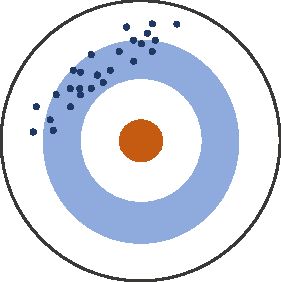
\includegraphics[scale=0.75]{norm_before.pdf}
        \end{minipage}
    }%
    \subfigure[After Normalization]{
        \begin{minipage}[t]{0.48\textwidth}
            \centering
            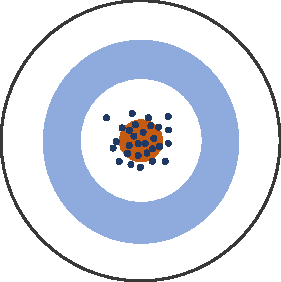
\includegraphics[scale=0.75]{norm_after.pdf}
        \end{minipage}
    }%
    \centering
    \caption{Normalization}
    \label{fig:normalization}
\end{figure}

在 python 中,可以很方便地实现输入数据的归一化
\begin{python}
X -= np.mean(X, axis=0)
X /= np.std(X, axis=0)
\end{python}

%%%
\section{Optimization Algorithms}

%%%%
\subsection{Mini-batch Gradient Descent}
\index{Mini-batch Gradient Descent}

之前的梯度下降算法都是基于整个训练集的,即每次迭代都要计算整个训练集的代价函数和梯度,然后更新权重和偏置。
这样的梯度下降算法称为\textbf{批量梯度下降(Batch Gradient Descent)},其缺点是每次更新梯度都需要完整遍历整个训练集,计算量很大,效率很低。
一种更好的方法是将训练集分成若干个子集,每次迭代只计算一个子集的代价函数和梯度,然后更新权重和偏置。
这样的梯度下降算法称为\textbf{小批量梯度下降(Mini-batch Gradient Descent)}。

\begin{hint}
    权重$W$和偏置$b$的规模完全由各层节点数$n^{[l]},\; 0 \leqslant l \leqslant L$决定,与样本数$m$无关。对于不同的样本数$m$,只需要调整$X$和$Y$的规模即可,而网络内部的节点数不需要调整就能适应不同规模的样本。
    这也是 Mini-batch 优化算法能实现的基础。
\end{hint}

在实现时,设定一个 \verb|mini_batch_size| (可简写为 \verb|batch_size|) ,将训练集打乱顺序,然后将其分成若干个大小为 \verb|batch_size| 的子集。
对于不同的 \verb|mini_batch| ,仍共享相同的权重和偏置,即训练的仍是同一个网络。

前向传播的过程与之前的算法相同,相当于将第$t$个子集$X^{\{t\}}$作为输入矩阵,依次计算出各层的输出矩阵$A^{[l]}$。
应当注意,此时输入的样本的规模相当于从$m$变成了 \verb|batch_size|,在计算代价函数时需要除以 \verb|batch_size| 而不是$m$。例如在使用 $L_2$ 正则化时,代价函数的计算公式为
\begin{equation}
    J^{\{t\}} = \frac{1}{\mathtt{batch\_size}}\sum_{i=1}^\mathtt{batch\_size} L(\hat{y}^{(i)}, y^{(i)}) + \frac{\lambda}{2\;\mathtt{batch\_size}}\sum_{l=1}^L||W^{[l]}||_{\mathrm{F}}^2
\end{equation}
不同的 \verb|mini_batch| 包含不同的样本,因此即使使用同样的权重和偏置,不同的 \verb|mini_batch| 也会得到不同的代价函数。
在使用小批量梯度下降时,代价函数并不是像之前那样单调递减的,而是有一定的波动。

\begin{figure}[h!bt]
    \centering
    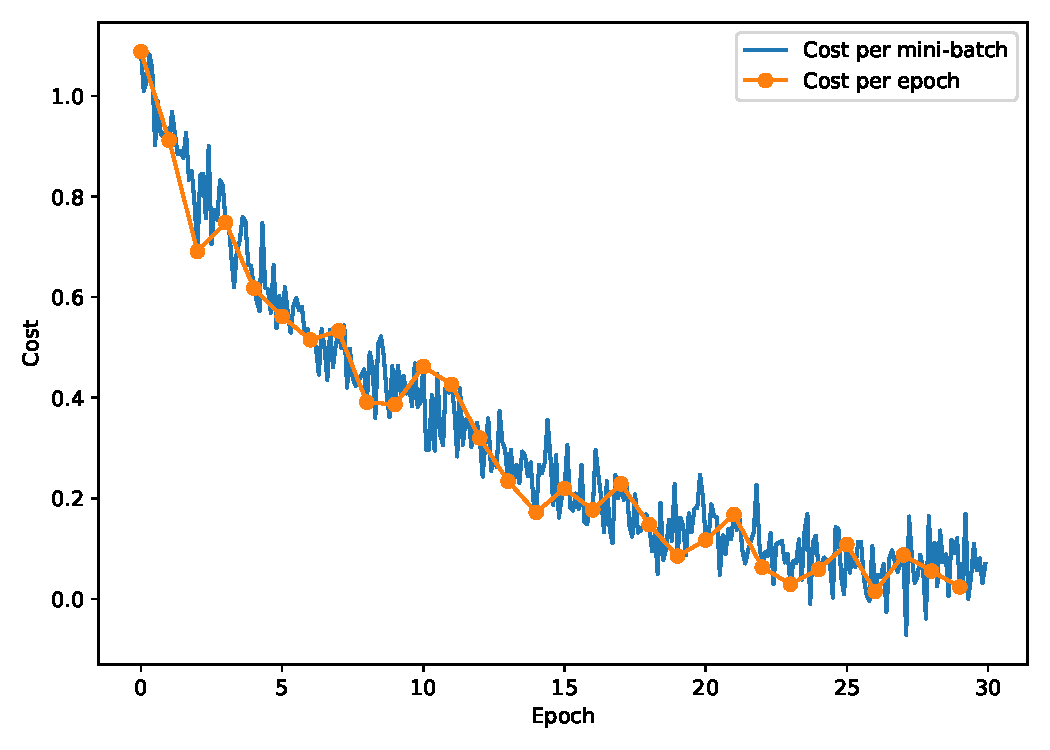
\includegraphics[scale=0.65]{mini-batch_cost.pdf}
    \caption{Cost Function in Mini-batch Gradient Descent}
    \label{fig:mini-batch_cost}
\end{figure}

反向传播的过程也与之前的算法相同,依次计算出各层的梯度矩阵$\d W^{[l]}$和$\d b^{[l]}$,然后更新权重和偏置。

当所有的 \verb|mini_batch| 都遍历完一遍训练集后,称为完成了一个 \texttt{\textbf{epoch}}。
训练过程中使用的 \verb|epoch| 数也是一个超参数,表示了整个训练集被遍历的次数。在每个 \verb|epoch| 结束后,可以重新打乱训练集的顺序,然后再次分成若干个 \verb|mini_batch| 继续训练以增强随机性。

当数据量非常大时,使用小批量梯度下降算法已被证明是一种有效的优化算法,可以加快训练速度。
小批量梯度下降算法每次更新权重和偏置只需要计算一个 \verb|mini_batch| 的代价函数和梯度,相比于批量梯度下降算法大大减少了计算量,可以更快地收敛。

\verb|batch_size| 的取值一般为2的幂次方,如32、64、128等,一般不会超过512。过大的 \verb|batch_size| 会导致训练速度变慢,而过小的 \verb|batch_size| 会导致训练过程中的代价函数波动较大。

%%%%
\subsection{Gradient Descent with Momentum}

在讨论矩估计时,符号标记忽略了层数$l$便于书写,但在实际实现时,应当使用$l$来区分不同层的矩估计。

动量可以平均梯度的方向,从而减少梯度下降的震荡。

一般不删除系数 $1 - \beta$ 
